% ============================================================
%  Presentation slides for
%  "Qubit Mapping for Fault-Tolerant Compilation:
%   A Gaussian Potential-Field Placement Heuristic"
%  Target talk length: 10-15 minutes.
%  Compile with: pdflatex slides.tex   (run twice for refs)
% ============================================================
\documentclass[aspectratio=169,10pt]{beamer}

% ── Packages ─────────────────────────────────────────────────
\usepackage[T1]{fontenc}
\usepackage[utf8]{inputenc}
\usepackage{amsmath,amssymb}
\usepackage{booktabs}
\usepackage{graphicx}
\usepackage{tikz}
\usepackage{pgfplots}
\pgfplotsset{compat=1.18}
\usetikzlibrary{positioning,arrows.meta,calc,shapes.geometric,
                backgrounds,fit,decorations.pathmorphing,patterns,
                shapes.misc}
\newcommand{\M}{\mathcal{M}}

% ── Palette ──────────────────────────────────────────────────
\definecolor{ftblue}{HTML}{1F4E79}
\definecolor{ftorange}{HTML}{E8820C}
\definecolor{ftgreen}{HTML}{2E8B57}
\definecolor{ftred}{HTML}{C0392B}
\definecolor{ftgray}{HTML}{555555}
\definecolor{ftbg}{HTML}{F4F6F8}

% ── Minimal clean theme (pdflatex-safe, no external fonts) ───
\usefonttheme{professionalfonts}
\setbeamertemplate{navigation symbols}{}
\setbeamercolor{frametitle}{fg=ftblue}
\setbeamercolor{title}{fg=ftblue}
\setbeamercolor{structure}{fg=ftblue}
\setbeamercolor{normal text}{fg=black}
\setbeamercolor{itemize item}{fg=ftorange}
\setbeamercolor{itemize subitem}{fg=ftorange}
\setbeamercolor{block title}{fg=white,bg=ftblue}
\setbeamercolor{block body}{bg=ftblue!8}
\setbeamerfont{frametitle}{series=\bfseries}
\setbeamerfont{title}{series=\bfseries}

\setbeamertemplate{frametitle}{%
    \vspace*{0.55em}%
    \usebeamercolor[fg]{frametitle}\large\insertframetitle\par
    \vspace{-0.28em}{\color{ftorange}\rule{\textwidth}{1.1pt}}\par
}
\setbeamertemplate{footline}{%
    \hbox{}\hfill
    {\color{ftgray}\footnotesize Gaussian Field Placement for FT Compilation}\hfill
    {\color{ftblue}\footnotesize\insertframenumber}\hspace{1em}\vspace{0.5em}%
}
\setbeamertemplate{itemize item}{\small\raise0.5pt\hbox{\textbullet}}

% ── Reusable TikZ styles ─────────────────────────────────────
\tikzset{
  tile/.style   ={draw=ftgray!55, minimum size=6mm, inner sep=0pt},
  data/.style   ={tile, fill=ftblue!25, draw=ftblue, rounded corners=1pt},
  magic/.style  ={tile, fill=ftorange!85, draw=ftorange!55!black},
  free/.style   ={tile, fill=white},
  corridor/.style={tile, fill=ftgreen!35, draw=ftgreen!55!black},
  forbid/.style ={tile, fill=ftred!18, draw=ftred!55, densely dashed},
  mstar/.style  ={star, star points=5, star point ratio=2.3, fill=white,
                  draw=ftorange!50!black, minimum size=3.2mm, inner sep=0pt, line width=0.3pt},
  qlabel/.style ={font=\scriptsize\bfseries, text=ftblue!75!black},
  pin/.style    ={-{Stealth[length=2mm]}, thick, shorten >=3mm, shorten <=3mm},
}
% draws a W x H lattice of free tiles at integer coords
\newcommand{\latgrid}[2]{%
  \foreach \xx in {0,...,#1}\foreach \yy in {0,...,#2}{%
     \node[free] at (\xx,\yy) {};}}

% ── Title metadata ───────────────────────────────────────────
\title{\bfseries Qubit Mapping for Fault-Tolerant Compilation}
\subtitle{A Gaussian Potential-Field Placement Heuristic}
\author{Alessandro Ruzza \and Federico Quartieri \and Daniele Salvi}
\institute{Politecnico di Milano}
\date{IEEE Quantum Week (QCE) 2026}

% ============================================================
\begin{document}

% ---------- TITLE ----------
{\setbeamertemplate{footline}{}
\begin{frame}[plain]
  \vspace{0.3cm}
  \begin{center}
  {\color{ftblue}\Large\bfseries Qubit Mapping for Fault-Tolerant Compilation}\\[4pt]
  {\color{ftorange}\large A Gaussian Potential-Field Placement Heuristic}\\[2pt]
  {\color{ftorange}\rule{0.6\textwidth}{1pt}}
  \end{center}

  \vspace{0.1cm}
  \begin{center}
  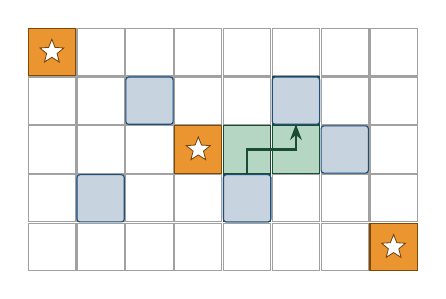
\begin{tikzpicture}[scale=0.62]
    % mini lattice with magic states + a routed corridor
    \latgrid{7}{4}
    % data patches
    \foreach \p in {(1,1),(2,3),(4,1),(5,3),(6,2)}
        \node[data] at \p {};
    % corridor highlight
    \foreach \c in {(4,1),(4,2),(5,2),(5,3)}
        \node[corridor] at \c {};
    \node[data] at (4,1) {}; \node[data] at (5,3) {};
    % magic states
    \node[magic] at (0,4) {}; \node[mstar] at (0,4){};
    \node[magic] at (7,0) {}; \node[mstar] at (7,0){};
    \node[magic] at (3,2) {}; \node[mstar] at (3,2){};
    \draw[pin, ftgreen!55!black] (4,1)--(4,2)--(5,2)--(5,3);
  \end{tikzpicture}
  \end{center}

  \vspace{0.15cm}
  \begin{center}
  {\bfseries Alessandro Ruzza \quad Federico Quartieri \quad Daniele Salvi}\\[2pt]
  {\color{ftgray}\small Politecnico di Milano \;\textbar\; IEEE Quantum Week (QCE) 2026}
  \end{center}
\end{frame}}

% ---------- 1. THE SETTING ----------
\begin{frame}{Fault-tolerant hardware: a 2D lattice of patches}
  \begin{columns}[c]
  \begin{column}{0.54\textwidth}
    \centering
    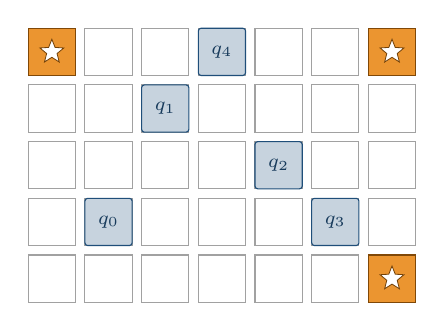
\begin{tikzpicture}[scale=0.72]
      \latgrid{6}{4}
      % data patches
      \foreach \p/\n in {(1,1)/q_0,(2,3)/q_1,(4,2)/q_2,(5,1)/q_3,(3,4)/q_4}{
          \node[data] at \p {};
          \node[qlabel] at \p {$\n$};}
      % magic tiles
      \foreach \m in {(0,4),(6,0),(6,4)}{
          \node[magic] at \m {}; \node[mstar] at \m {};}
    \end{tikzpicture}
  \end{column}
  \begin{column}{0.46\textwidth}
    \footnotesize
    \begin{itemize}
      \item Surface-code processor $=$ grid of \alert{patches}
      \item \textcolor{ftblue}{\rule{2.2mm}{2.2mm}}~ \textbf{data patch} $=$ one logical qubit
      \item[] \tikz\node[free,scale=0.55]{};~ \textbf{free tile} $=$ ancilla, reset each step
      \item \textcolor{ftorange}{$\star$}~ \textbf{magic state} $=$ fuel for $T$ gates
    \end{itemize}
    \vspace{2pt}
    \begin{block}{Two coupled jobs}
      \footnotesize
      \textbf{Map:} place qubits on tiles \\
      \textbf{Route:} schedule lattice surgery
    \end{block}
  \end{column}
  \end{columns}
\end{frame}

% ---------- 2. GATES = SURGERY ----------
\begin{frame}{Gates run by \emph{lattice surgery}, not SWAP}
  \centering
  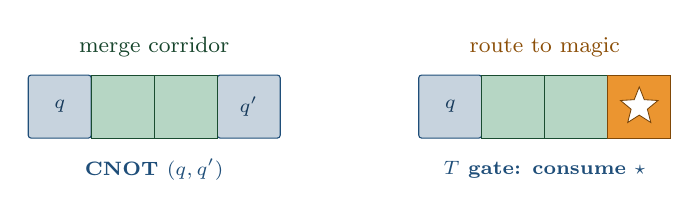
\begin{tikzpicture}[scale=0.8]
    % --- 2-qubit gate via merged corridor ---
    \begin{scope}
      \node[data,minimum size=8mm] (a) at (0,0) {}; \node[qlabel] at (a){$q$};
      \node[data,minimum size=8mm] (b) at (3,0) {}; \node[qlabel] at (b){$q'$};
      \foreach \i in {1,2}\node[corridor,minimum size=8mm] at (\i,0){};
      \node[font=\footnotesize,ftgreen!50!black] at (1.5,0.95){merge corridor};
      \node[font=\scriptsize\bfseries,ftblue] at (1.5,-1.0){CNOT $(q,q')$};
    \end{scope}
    % --- T gate via magic state path ---
    \begin{scope}[xshift=6.2cm]
      \node[data,minimum size=8mm] (c) at (0,0) {}; \node[qlabel] at (c){$q$};
      \foreach \i in {1,2}\node[corridor,minimum size=8mm] at (\i,0){};
      \node[magic,minimum size=8mm] (m) at (3,0){}; \node[mstar,minimum size=5mm] at (3,0){};
      \node[font=\footnotesize,ftorange!60!black] at (1.5,0.95){route to magic};
      \node[font=\scriptsize\bfseries,ftblue] at (1.5,-1.0){$T$ gate: consume $\star$};
    \end{scope}
  \end{tikzpicture}

  \vspace{0.5cm}
  
\begin{tikzpicture}
    \node[draw=ftorange,fill=ftorange!10,rounded corners,inner sep=6pt,font=\small]{
      \textbf{Scarce resource is free \emph{space}} for corridors --- not the edges of a fixed coupling graph.};
  \end{tikzpicture}
\end{frame}

% ---------- 3. NISQ vs FT ----------
\begin{frame}{Why the NISQ cost model doesn't transfer}
  \centering
  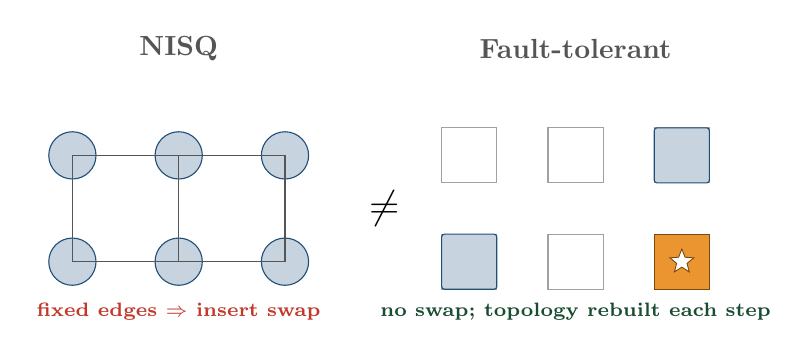
\begin{tikzpicture}[scale=0.9]
    % --- NISQ side ---
    \begin{scope}
      \node[font=\bfseries,ftgray] at (1.5,3.0){NISQ};
      % fixed coupling graph
      \foreach \p in {(0,0),(1.5,0),(3,0),(0,1.5),(1.5,1.5),(3,1.5)}
          \node[circle,fill=ftblue!25,draw=ftblue,minimum size=6mm] at \p {};
      \draw[ftgray] (0,0)--(1.5,0)--(3,0) (0,1.5)--(1.5,1.5)--(3,1.5)
                    (0,0)--(0,1.5) (1.5,0)--(1.5,1.5) (3,0)--(3,1.5);
      \node[ftred,font=\scriptsize\bfseries] at (1.5,-0.7){fixed edges $\Rightarrow$ insert \textsc{swap}};
    \end{scope}
    % arrow
    \node at (4.4,0.75){\Large$\neq$};
    % --- FT side ---
    \begin{scope}[xshift=5.6cm]
      \node[font=\bfseries,ftgray] at (1.5,3.0){Fault-tolerant};
      \foreach \xx in {0,1,2}\foreach \yy in {0,1}
          \node[free,minimum size=7mm] at (\xx*1.5,\yy*1.5){};
      \foreach \p in {(0,0),(3,1.5)}\node[data,minimum size=7mm] at \p {};
      \node[magic,minimum size=7mm] at (3,0){}; \node[mstar] at (3,0){};
      \node[ftgreen!55!black,font=\scriptsize\bfseries] at (1.5,-0.7){no \textsc{swap}; topology rebuilt each step};
    \end{scope}
  \end{tikzpicture}

  \vspace{0.45cm}
  \footnotesize
  \begin{tabular}{l c c}
    \toprule
        & \textbf{NISQ} & \textbf{Fault-tolerant} \\
    \midrule
    Bottleneck   & \textsc{swap} count           & routing \alert{corridors} \\
    Topology     & fixed coupling graph          & reconfigured every step \\
    Scarce thing & graph edges                   & free \alert{space} + magic access \\
    \bottomrule
  \end{tabular}
\end{frame}

% ---------- 4. PLACEMENT MATTERS ----------
\begin{frame}{A good \emph{placement} decides everything downstream}
  \begin{columns}[T]
  \begin{column}{0.4\textwidth}
    \centering {\color{ftred}\bfseries Bad: $T$-heavy qubit far from $\star$}\\[4pt]
    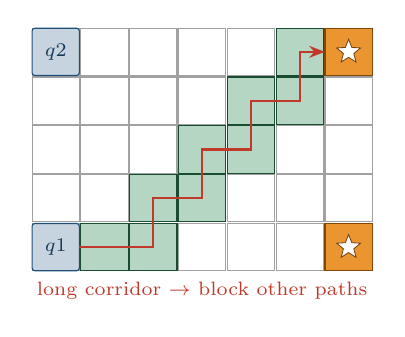
\begin{tikzpicture}[scale=0.62]
      \latgrid{6}{4}
      \node[data] at (0,0){}; \node[qlabel] at (0,0){$q1$};
      \node[data] at (0,4){}; \node[qlabel] at (0,4){$q2$};
      \node[magic] at (6,4){}; \node[mstar] at (6,4){};
      \node[magic] at (6,0){}; \node[mstar] at (6,0){};
      \foreach \c in {(1,0),(2,0),(2,1),(3,1),(3,2),(4,2),(4,3),(5,3),(5,4)}
        \node[corridor] at \c{};
      \draw[pin,ftred,thick]
        (0,0)--(2,0)--(2,1)--(3,1)--(3,2)--(4,2)--(4,3)--(5,3)--(5,4)--(6,4);
      \node[ftred,font=\scriptsize] at (3,-0.9){long corridor $\to$ block other paths};
    \end{tikzpicture}
  \end{column}
  \begin{column}{0.1\textwidth}
    \centering
    Circuit\\[5pt]
    T q1 \\[5pt]
    T q2
  \end{column}
  \begin{column}{0.4\textwidth}
    \centering {\color{ftgreen!55!black}\bfseries Good: $q$ hugs its $\star$}\\[4pt]
    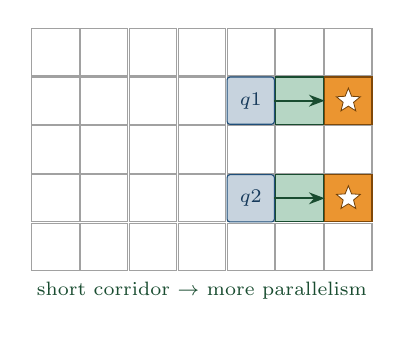
\begin{tikzpicture}[scale=0.62]
      \latgrid{6}{4}
      \node[data] at (4,3){}; \node[qlabel] at (4,3){$q1$};
      \node[data] at (4,1){}; \node[qlabel] at (4,1){$q2$};
      \node[magic] at (6,3){}; \node[mstar] at (6,3){};
      \node[magic] at (6,1){}; \node[mstar] at (6,1){};
      \node[corridor] at (5,3){};
      \node[corridor] at (5,1){};
      \draw[pin,ftgreen!55!black,thick] (4,3) -- (6,3);
      \draw[pin,ftgreen!55!black,thick] (4,1) -- (6,1);
      \node[ftgreen!55!black,font=\scriptsize] at (3,-0.9){short corridor $\to$ more parallelism};
    \end{tikzpicture}
  \end{column}
  \end{columns}

  \vspace{0.35cm}
  \centering
  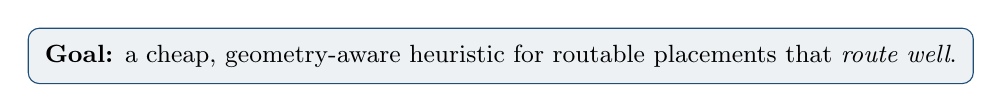
\begin{tikzpicture}
    \node[draw=ftblue,fill=ftblue!8,rounded corners,inner sep=6pt,font=\small]{
      \textbf{Goal:} a cheap, geometry-aware heuristic for routable placements that \emph{route well}.};
  \end{tikzpicture}
\end{frame}

% ---------- 5. KEY IDEA ----------
\begin{frame}{Key idea: placement as a \emph{potential field}}
  \begin{columns}[c]
  \begin{column}{0.46\textwidth}
    \footnotesize
    Borrow from robot motion planning:
    \begin{itemize}
      \item \textcolor{ftorange}{\textbf{Attract}} toward goals\\(magic states, partners)
      \item \textcolor{ftblue}{\textbf{Repel}} from obstacles\\(already-placed patches)
    \end{itemize}
    \vspace{4pt}
    Each qubit $\to$ a scalar \alert{score surface} over tiles.\\[3pt]
    Place it at the \textbf{safe maximum}.
  \end{column}
  \begin{column}{0.54\textwidth}
    \centering
    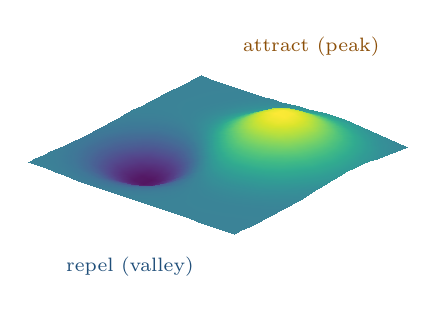
\begin{tikzpicture}
      \begin{axis}[width=6.4cm,height=4.6cm,
          domain=-3:3,y domain=-3:3,samples=24,
          view={40}{55},colormap/viridis,
          axis lines=none,ticks=none,clip=false]
        \addplot3[surf,shader=interp,fill opacity=0.92]
          {1.6*exp(-((x-1)^2+(y-1)^2)/2.2)
           - 1.1*exp(-((x+1.2)^2+(y+1)^2)/1.3)};
      \end{axis}
      \node[font=\scriptsize,ftorange!60!black] at (3.6,2.8){attract (peak)};
      \node[font=\scriptsize,ftblue] at (1.3,0){repel (valley)};
    \end{tikzpicture}
  \end{column}
  \end{columns}
\end{frame}

% ---------- 6. ONE FIELD ----------
\begin{frame}{One influence field $=$ a 2D Gaussian}
  \begin{columns}[c]
  \begin{column}{0.5\textwidth}
    \small
    \[ g(x,y)=w\,\exp\!\Big(\!-\tfrac{(x-\mu_x)^2}{2\sigma_x^2}-\tfrac{(y-\mu_y)^2}{2\sigma_y^2}\Big) \]
    \begin{itemize}\footnotesize
      \item \textbf{Attractive:} add $g$
      \item \textbf{Repulsive:} add valley $\max(w-g,\,0)$
    \end{itemize}
    \vspace{4pt}
    One knob --- \alert{confidence} $\kappa\in(0,1)$:
    \[ \sigma=\frac{R}{\sqrt{-2\ln(1-\kappa)}} \]
    {\footnotesize keeps fraction $(1-\kappa)$ of the peak at range $R$.\\ Larger $\kappa$ $\to$ broader reach.}
  \end{column}
  \begin{column}{0.5\textwidth}
    \centering
    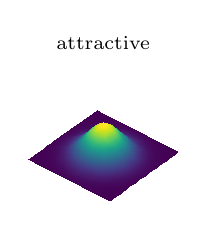
\begin{tikzpicture}
      \begin{axis}[width=3.5cm,height=3.2cm,domain=-3:3,y domain=-3:3,
          samples=22,view={40}{60},axis lines=none,ticks=none,
          colormap/viridis,title={\scriptsize attractive}]
        \addplot3[surf,shader=interp]{exp(-(x^2+y^2)/2)};
      \end{axis}
    \end{tikzpicture}\hspace{-0.3cm}
    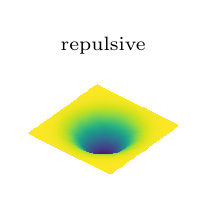
\begin{tikzpicture}
      \begin{axis}[width=3.5cm,height=3.2cm,domain=-3:3,y domain=-3:3,
          samples=22,view={40}{60},axis lines=none,ticks=none,
          colormap/viridis,title={\scriptsize repulsive}]
        \addplot3[surf,shader=interp]{1-exp(-(x^2+y^2)/2)};
      \end{axis}
    \end{tikzpicture}
  \end{column}
  \end{columns}
\end{frame}

% ---------- 7. FOUR FAMILIES ----------
\begin{frame}{Four field families superpose into the score $S$}
  \centering
  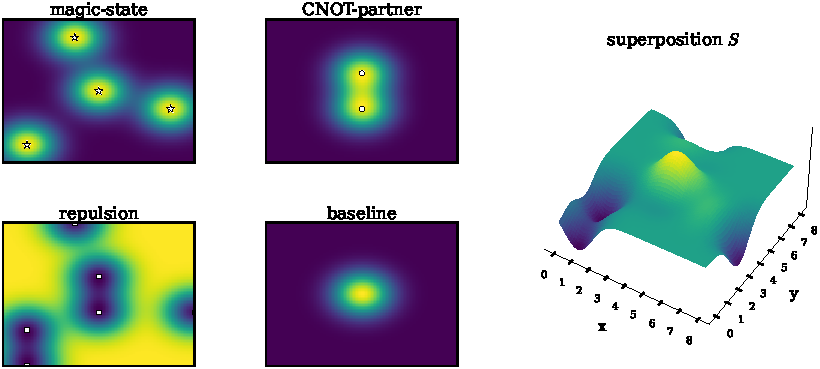
\includegraphics[width=0.8\linewidth]{figures/gaussian_fields.pdf}

  \vspace{0.1cm}
  \footnotesize
  \[ S(v)=\underbrace{\textstyle\sum_{m}g^{\mathrm{mag}}_m}_{\textcolor{ftorange}{\star\ \text{$T$ demand}}}
        +\underbrace{\textstyle\sum_{p}g^{\mathrm{cnot}}_p}_{\textcolor{ftblue}{\circ\ \text{partners}}}
        +\underbrace{\textstyle\sum_{u}g^{\mathrm{rep}}_u}_{\square\ \text{spread out}}
        +\underbrace{b(v)}_{\text{center}} \]
  \vspace{2pt}\par
  Place $q$ at the \textcolor{ftred}{\textbf{safe maximum}} of $S$ (red dot, right).
\end{frame}

% ---------- 8. SAFE PASSAGE ----------
\begin{frame}{Safe passage: never \emph{trap} a patch}
  \footnotesize Reject any placement that blocks a committed patch from its partners or a magic state.
  \vspace{0.2cm}
  \begin{columns}[T]
  \begin{column}{0.5\textwidth}
    \centering {\bfseries\color{ftblue} Cube} \;(default)\\[3pt]
    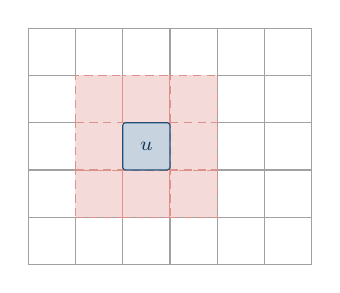
\begin{tikzpicture}[scale=0.6]
      \latgrid{5}{4}
      \node[data] at (2,2){}; \node[qlabel] at (2,2){$u$};
      \foreach \dx in {-1,0,1}\foreach \dy in {-1,0,1}{
        \pgfmathtruncatemacro{\cx}{2+\dx}\pgfmathtruncatemacro{\cy}{2+\dy}
        \ifnum\dx=0\ifnum\dy=0\else\node[forbid] at (\cx,\cy){};\fi
        \else\node[forbid] at (\cx,\cy){};\fi}
      \node[data] at (2,2){}; \node[qlabel] at (2,2){$u$};
    \end{tikzpicture}\\[2pt]
    {\scriptsize forbid the $3\times3$ ring $\Rightarrow$ bigger grid,\\ \textbf{shorter routes}}
  \end{column}
  \begin{column}{0.5\textwidth}
    \centering {\bfseries\color{ftgreen!55!black} Connectivity}\\[3pt]
    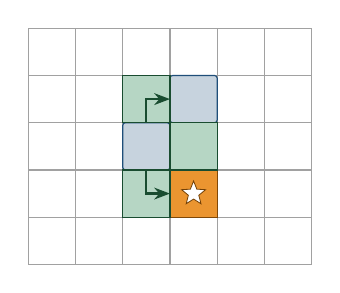
\begin{tikzpicture}[scale=0.6]
      \latgrid{5}{4}
      \node[data] at (2,2){}; \node[data] at (3,3){};
      \node[magic] at (3,1){}; \node[mstar] at (3,1){};
      \foreach \c in {(2,3),(2,1),(3,2)}
        \node[corridor] at \c{};
      \draw[pin,ftgreen!55!black] (2,2)--(2,3)--(3,3);
      \draw[pin,ftgreen!55!black] (2,2)--(2,1)--(3,1);
    \end{tikzpicture}\\[2pt]
    {\scriptsize admit if reachability still holds $\Rightarrow$\\ \textbf{packs tightly}, smaller area}
  \end{column}
  \end{columns}
\end{frame}

% ---------- 9. COARSE vs FINE ----------
\begin{frame}{Two weightings: coarse vs.\ fine}
  \centering
  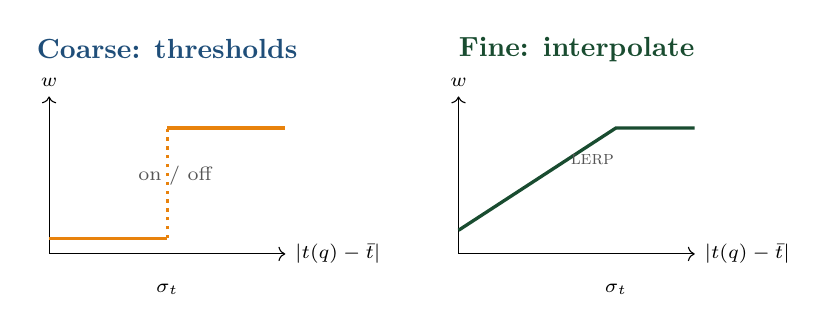
\begin{tikzpicture}[scale=1]
    % coarse: step
    \begin{scope}
      \node[font=\bfseries,ftblue] at (1.5,2.6){Coarse: thresholds};
      \draw[->] (0,0)--(3,0) node[right,font=\scriptsize]{$|t(q)-\bar t|$};
      \draw[->] (0,0)--(0,2) node[above,font=\scriptsize]{$w$};
      \draw[ftorange,very thick] (0,0.2)--(1.5,0.2);
      \draw[ftorange,very thick] (1.5,1.6)--(3,1.6);
      \draw[ftorange,very thick,dotted] (1.5,0.2)--(1.5,1.6);
      \node[font=\scriptsize] at (1.5,-0.45){$\sigma_t$};
      \node[font=\scriptsize,ftgray] at (1.6,1.0){on / off};
    \end{scope}
    % fine: lerp
    \begin{scope}[xshift=5.2cm]
      \node[font=\bfseries,ftgreen!55!black] at (1.5,2.6){Fine: interpolate};
      \draw[->] (0,0)--(3,0) node[right,font=\scriptsize]{$|t(q)-\bar t|$};
      \draw[->] (0,0)--(0,2) node[above,font=\scriptsize]{$w$};
      \draw[ftgreen!55!black,very thick] (0,0.3)--(2,1.6)--(3,1.6);
      \node[font=\scriptsize] at (2,-0.45){$\sigma_t$};
      \node[font=\scriptsize,ftgray] at (1.7,1.2){\textsc{lerp}};
    \end{scope}
  \end{tikzpicture}

  \vspace{0.4cm}
  \footnotesize
  \begin{itemize}
    \item Same fields --- only \textbf{how weights \& signs come from circuit stats} differs.
    \item Sign: \textcolor{ftorange}{attract} if $T$-heavy, \textcolor{ftblue}{repel} if $T$-light (free the magic neighbourhood).
    \item \textbf{Fine} reacts smoothly to deviation from the circuit's average profile.
  \end{itemize}
\end{frame}

% ---------- 10. ALGORITHM ----------
\begin{frame}{The placement loop}
  \centering
  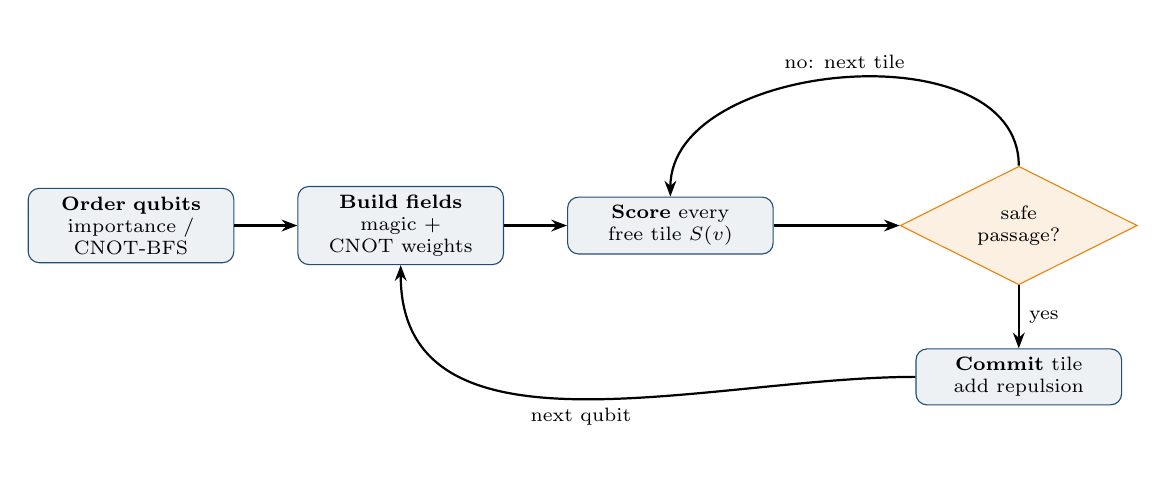
\begin{tikzpicture}[node distance=5mm and 8mm,font=\scriptsize,
      box/.style={draw=ftblue,fill=ftblue!8,rounded corners,
                  text width=2.4cm,align=center,minimum height=7mm,inner sep=3pt},
      dec/.style={draw=ftorange,fill=ftorange!12,diamond,aspect=2,
                  align=center,inner sep=1pt,text width=1.8cm},
      fl/.style={-{Stealth[length=2mm]},thick}]
    \node[box] (order) {\textbf{Order qubits}\\importance / CNOT-BFS};
    \node[box,right=of order] (build){\textbf{Build fields}\\magic + CNOT weights};
    \node[box,right=of build] (score){\textbf{Score} every\\free tile $S(v)$};
    \node[dec,right=16mm of score] (safe){safe\\passage?};
    \node[box,below=8mm of safe] (commit){\textbf{Commit} tile\\add repulsion};
    \draw[fl] (order)--(build);
    \draw[fl] (build)--(score);
    \draw[fl] (score)--(safe);
    \draw[fl] (safe)-- node[right,font=\scriptsize]{yes} (commit);
    \draw[fl] (safe.north) to[out=90,in=90] node[above,font=\scriptsize]{no: next tile}(score.north);
    \draw[fl] (commit.west) to[out=180,in=270] node[below,font=\scriptsize]{next qubit}(build.south);
  \end{tikzpicture}

  \vspace{0.15cm}
  \footnotesize
  \begin{columns}[T]
    \begin{column}{0.5\textwidth}
      \textbf{Importance first:} $t(q)+c_{\max}(q)$ --- constrain the lattice while empty.
    \end{column}
    \begin{column}{0.5\textwidth}
      \textbf{CNOT-BFS} (sparse, $\rho<\tau$): strongest partner already placed.
    \end{column}
  \end{columns}

  \vspace{4pt}
  \centering{\scriptsize Per qubit $O(|V|\,(|V_{\mathrm m}|+|P(q)|+|\M|))$ $\Rightarrow$ low-order polynomial.}
\end{frame}

% ---------- 11. FORMATION ----------
\begin{frame}{A mapping forming, qubit by qubit}
  \centering
  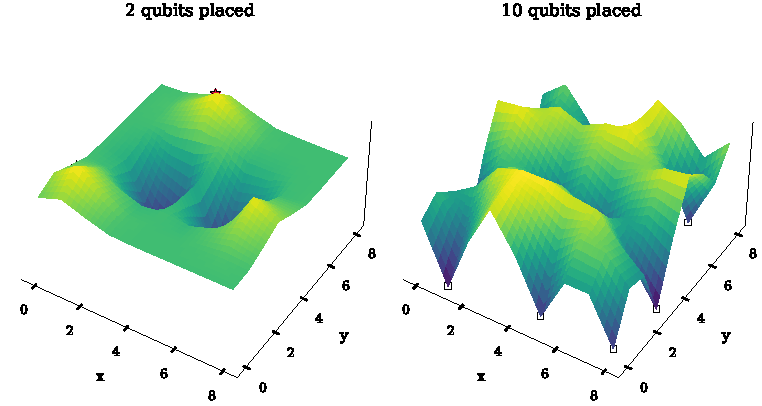
\includegraphics[width=0.86\linewidth]{figures/gaussian_frames.pdf}

  \vspace{0.1cm}
  \footnotesize
  Repulsion carves a \textbf{well} at every committed patch (white $\square$),
  spacing qubits apart while peaks stay near magic tiles ($\star$).
\end{frame}

% ---------- 12. EVALUATION ----------
\begin{frame}{Evaluation}
  \begin{columns}[T]
  \begin{column}{0.52\textwidth}
    \footnotesize
    \textbf{Implementation} --- open-source C++20
    \begin{itemize}
      \item OpenQASM front-end
      \item Gaussian mapper $+$ lattice-surgery router
      \item auto-sized lattice \& magic budget
    \end{itemize}
    \vspace{4pt}
    \textbf{Benchmarks} --- arithmetic, algorithmic, state-prep families\\
    {\scriptsize \texttt{adder}, \texttt{qft}, \texttt{multiplier}, \texttt{hhl}, \texttt{factor247}, \texttt{ising}, \dots}
  \end{column}
  \begin{column}{0.48\textwidth}
    \footnotesize
    \textbf{Baselines}
    \begin{itemize}
      \item \textcolor{ftgray}{\textbf{Random}} --- cheap, $3{\times}3$-spaced restarts; keep best
      \item \textcolor{ftgray}{\textbf{WISQ}} --- external FT compiler
    \end{itemize}
    \vspace{4pt}
    \textbf{Metrics}
    \begin{itemize}
      \item routing \alert{steps} (surgery time-depth)
      \item compilation time
      \item avg.\ parallelism
    \end{itemize}
  \end{column}
  \end{columns}

  \vspace{0.25cm}
  \centering
  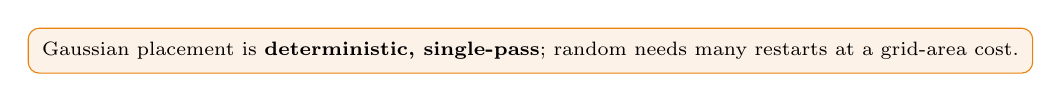
\begin{tikzpicture}
    \node[draw=ftorange,fill=ftorange!10,rounded corners,inner sep=5pt,font=\scriptsize]{
      Gaussian placement is \textbf{deterministic, single-pass}; random needs many restarts at a grid-area cost.};
  \end{tikzpicture}
\end{frame}

% ---------- 13. RESULTS (schematic) ----------
\begin{frame}{Results: reading the scatter}
  \begin{columns}[c]
  \begin{column}{0.52\textwidth}
    \centering
    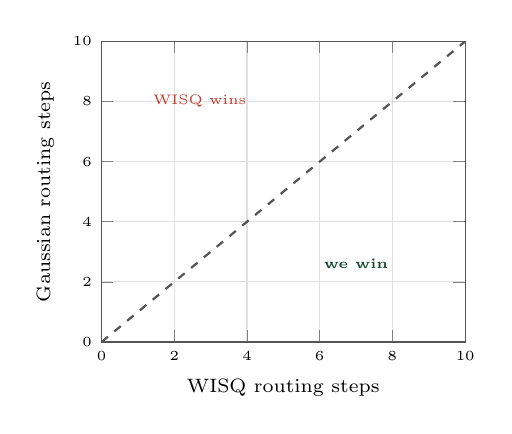
\begin{tikzpicture}
      \begin{axis}[width=6.2cm,height=5.4cm,
          xlabel={\scriptsize WISQ routing steps},
          ylabel={\scriptsize Gaussian routing steps},
          xmin=0,xmax=10,ymin=0,ymax=10,
          tick label style={font=\tiny},
          axis line style={ftgray},grid=both,
          grid style={ftgray!18}]
        \addplot[domain=0:10,ftgray,dashed,thick]{x};
        \node[ftgreen!55!black,font=\tiny] at (axis cs:7,2.6){\textbf{we win}};
        \node[ftred,font=\tiny] at (axis cs:2.7,8){WISQ wins};
        % \addplot[only marks,mark=*,ftblue,mark size=1.6pt]
        %   coordinates {(3,2)(5,3.4)(6,4)(8,5)(4,3)(7,5.5)(9,6)(2.5,2)};
      \end{axis}
    \end{tikzpicture}
  \end{column}
  \begin{column}{0.48\textwidth}
    \footnotesize
    \begin{itemize}
      \item Each point $=$ one circuit.
      \item \textcolor{ftgreen!55!black}{\textbf{Below diagonal}} $\Rightarrow$ fewer routing steps than WISQ.
      \item WISQ entries also flag circuits where it \alert{times out / fails} but Gaussian completes.
    \end{itemize}
    \vspace{6pt}
    {\scriptsize\itshape Schematic --- full per-benchmark table \& numbers in the paper and artifact repository.}
  \end{column}
  \end{columns}
\end{frame}

% ---------- 14. CONCLUSION ----------
\begin{frame}{Takeaways}
  \begin{columns}[c]
  \begin{column}{0.58\textwidth}
    \begin{block}{Contribution}
      \footnotesize
      Fold $T$-locality, interaction clustering, and corridor preservation into \textbf{one additive Gaussian score}; place at the \textbf{safe maximum}.
    \end{block}
    \vspace{2pt}
    \footnotesize
    \textbf{Why it works}
    \begin{itemize}
      \item cheap, interpretable, deterministic
      \item safe-passage $\Rightarrow$ \emph{always routable}
      \item coarse / fine $\times$ cube / conn regimes
    \end{itemize}
    \vspace{4pt}
    \textbf{Next} --- learn the weights; feed field gradient back into the router so placement \& scheduling co-adapt.
  \end{column}
  \begin{column}{0.42\textwidth}
    \centering
    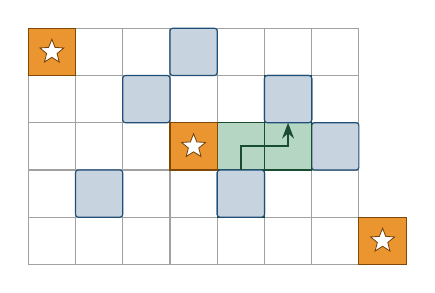
\begin{tikzpicture}[scale=0.6]
      \latgrid{6}{4}
      \foreach \p in {(1,1),(2,3),(4,1),(5,3),(6,2),(3,4)}\node[data] at \p {};
      \foreach \c in {(4,1),(4,2),(5,2),(5,3)}\node[corridor] at \c{};
      \node[data] at (4,1){}; \node[data] at (5,3){};
      \foreach \m in {(0,4),(7,0),(3,2)}{\node[magic] at \m{};\node[mstar] at \m{};}
      \draw[pin,ftgreen!55!black] (4,1)--(4,2)--(5,2)--(5,3);
    \end{tikzpicture}\\[4pt]
    {\scriptsize\color{ftgray} open source: \texttt{ftqc}}
  \end{column}
  \end{columns}
\end{frame}

% ---------- THANKS ----------
{\setbeamertemplate{footline}{}
\begin{frame}[plain]
  \centering
  \vspace{1.3cm}
  {\color{ftblue}\Large\bfseries Thank you!}\\[6pt]
  {\color{ftorange}\rule{0.4\textwidth}{1pt}}\\[10pt]
  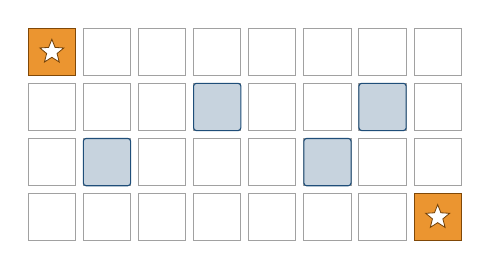
\begin{tikzpicture}[scale=0.7]
    \latgrid{7}{3}
    \foreach \p in {(1,1),(3,2),(5,1),(6,2)}\node[data] at \p {};
    \node[magic] at (0,3){};\node[mstar] at (0,3){};
    \node[magic] at (7,0){};\node[mstar] at (7,0){};
  \end{tikzpicture}\\[8pt]
  {\small Alessandro Ruzza \;\textbar\; Federico Quartieri \;\textbar\; Daniele Salvi}\\
  {\color{ftgray}\small Politecnico di Milano}
\end{frame}}

\end{document}
